% !TEX TS-program = pdflatex
% !TEX encoding = UTF-8 Unicode

\documentclass{beamer}
% for handouts: \documentclass[handout]{beamer}

%\setbeamertemplate{background canvas}[vertical shading][bottom=white,top=structure.fg!25]
% or whatever

\usetheme[compress]{Amsterdam}
%\setbeamertemplate{headline}{}
%\setbeamertemplate{footline}{}
%\setbeamersize{text margin left=0.5cm}
  
\usepackage[english]{babel}
\usepackage{listings}
\usepackage{geometry}
\usepackage{hyperref}

\usepackage{color}
\usepackage[T1]{fontenc}
\usepackage[utf8]{inputenc}
\usepackage{lmodern}

\usepackage{multicol}
\lstset{
basicstyle=\scriptsize\ttfamily,
columns=flexible,
breaklines=true,
numbers=left,
%stepsize=1,
numberstyle=\tiny,
backgroundcolor=\color[rgb]{0.85,0.90,1}
}


\begin{document}

\title[Big Data and Automated Content Analysis]{\textbf{Big Data and Automated Content Analysis} \\ Week 7 -- Wednesday \\ »Machine Learning«}
\author[Damian Trilling]{Joanna Strycharz \& Damian Trilling \\ ~ \\ \footnotesize{d.c.trilling@uva.nl \\@damian0604} \\ \url{www.damiantrilling.net}}
\date{23 May 2018}
\institute[UvA]{Afdeling Communicatiewetenschap \\Universiteit van Amsterdam}


\begin{frame}{}
\titlepage
\end{frame}

\begin{frame}{Today}
\tableofcontents
\end{frame}




\section[Recap]{Recap: Types of Automated Content Analysis}
\begin{frame}{}
Recap: Types of Automated Content Analysis
\end{frame}
\subsection*{Top-down vs. bottom-up}


%{\setbeamercolor{background canvas}{bg=black}
\begin{frame}[plain]
\makebox[\linewidth]{
\includegraphics[width=\paperwidth,height=\paperheight,keepaspectratio]{../../pictures//boumanstrilling2016}}
\end{frame}
%}




\begin{frame}{Some terminology }
	\begin{columns}[t]
		\column{.5\textwidth}
		
		\begin{block}<1-4>{Supervised machine learning}
			You have a dataset with both predictor and outcome (independent and dependent variables; features and labels) --- a \emph{labeled} dataset.
			\onslide<2>{
				\footnotesize{Think of regression: You measured \texttt{x1}, \texttt{x2}, \texttt{x3} and you want to predict \texttt{y}, which you also measured}}
		\end{block}
		
		\column{.5\textwidth}
		
		\begin{block}<3->{Unsupervised machine learning}
			You have no labels. \onslide<4>{(\footnotesize{You did not measure \texttt{y})}}\\
			\onslide<5>{\textbf{Again, you already know some techniques to find out how \texttt{x1}, \texttt{x2},\ldots \texttt{x\_i} co-occur from other courses:} \begin{itemize}
					\item Principal Component Analysis (PCA)
					\item Cluster analysis
					\item \ldots
				\end{itemize}
			}
		\end{block}
		
	\end{columns}
	
\end{frame}








\section{Unsupervised Machine Learning}
\begin{frame}[plain]
	inductive and bottom-up:\\ \textbf{unsupervised machine learning}\\
	\vspace{1cm}\hspace{1cm} \onslide<2> \footnotesize{(something you aready did in your Bachelor -- no kidding.)}
\end{frame}



\subsection{PCA}




\begin{frame}{Principal Component Analysis? How does \emph{that} fit in here?}
	\onslide<2>{In fact, PCA is used everywhere, even in image compression}
	
	\begin{block}<3->{PCA in ACA}
		\begin{itemize}
			\item Find out what word cooccur (inductive frame analysis)
			\item Basically, transform each document in a vector of word frequencies and do a PCA
		\end{itemize}
	\end{block}
	%\onslide<4>{\textbf{But we'll look at the state of the art instead: Latent Dirichlet Allication (LDA)}}
\end{frame}

\begin{frame}[fragile]{A so-called term-document-matrix}
\begin{lstlisting}
      w1,w2,w3,w4,w5,w6 ...
text1, 2, 0, 0, 1, 2, 3 ...
text2, 0, 0, 1, 2, 3, 4 ...
text3, 9, 0, 1, 1, 0, 0 ...
...
\end{lstlisting}
\vspace{1cm}
\onslide<2>{These can be simple counts, but also more advanced metrics, like tf-idf scores (where you weigh the frequency by the number of documents in which it occurs), cosine distances, etc.}
\end{frame}


\begin{frame}{PCA: implications and problems}
	\begin{itemize}
		\item given a term-document matrix, easy to do with any tool
		\item probably extremely skewed distributions
		\item some problematic assumptions: does the goal of PCA, to find a solution in which one word loads on \emph{one} component match real life, where a word can belong to several topics or frames?
	\end{itemize}
\end{frame}





\subsection{LDA}


\begin{frame}{}
	Enter \textbf{topic modeling with Latent Dirichlet Allocation (LDA)}
\end{frame}






\begin{frame}{LDA, what's that?}
	\begin{block}{No mathematical details here, but the general idea}
		\begin{itemize}
			\item There are $k$ topics, $T_1$\ldots$T_k$
			\item Each document $D_i$ consists of a mixture of these topics, e.g.$80\% T_1, 15\% T_2, 0\% T_3, \ldots 5\% T_k $
			\item On the next level, each topic consists of a specific probability distribution of words
			\item Thus, based on the frequencies of words in $D_i$, one can infer its distribution of topics
			\item Note that LDA (like PCA) is a Bag-of-Words (BOW) approach
		\end{itemize}
	\end{block}
	
\end{frame}




\begin{frame}[fragile]{Doing a LDA in Python}
You can use gensim ({\v R}eh{\r u}{\v r}ek \& Sojka, 2010) for this.

Let us assume you have a list of lists of words (!) called \texttt{texts}:

\begin{lstlisting}
articles=['The tax deficit is higher than expected. This said xxx ...', 'Germany won the World Cup. After a']
texts=[art.split() for art in articles]
\end{lstlisting}
which looks like this:
\begin{lstlisting}
[['The', 'tax', 'deficit', 'is', 'higher', 'than', 'expected.', 'This', 'said', 'xxx', '...'], ['Germany', 'won', 'the', 'World', 'Cup.', 'After', 'a']]
\end{lstlisting}

\tiny{{\v R}eh{\r u}{\v r}ek, R., \& Sojka, P. (2010). Software framework for topic modelling with large corpora. \emph{Proceedings of the LREC 2010 Workshop on New Challenges for NLP Frameworks}, pp. 45–50. Valletta, Malta: ELRA. }

\end{frame}




\begin{frame}[plain,fragile]
\begin{lstlisting}
from gensim import corpora, models

NTOPICS = 100
LDAOUTPUTFILE="topicscores.tsv"

# Create a BOW represenation of the texts
id2word = corpora.Dictionary(texts)
mm =[id2word.doc2bow(text) for text in texts]

# Train the LDA models.
mylda = models.ldamodel.LdaModel(corpus=mm, id2word=id2word, num_topics=NTOPICS, alpha="auto")

# Print the topics.
for top in mylda.print_topics(num_topics=NTOPICS, num_words=5):
  print ("\n",top)

print ("\nFor further analysis, a dataset with the topic score for each document is saved to",LDAOUTPUTFILE)

scoresperdoc=mylda.inference(mm)

with open(LDAOUTPUTFILE,"w",encoding="utf-8") as fo:
  for row in scoresperdoc[0]:
    fo.write("\t".join(["{:0.3f}".format(score) for score in row]))
fo.write("\n")
\end{lstlisting}

\end{frame}


\begin{frame}[fragile]{Output: Topics (below) \& topic scores (next slide)}
\begin{lstlisting}
0.069*fusie + 0.058*brussel + 0.045*europesecommissie + 0.036*europese + 0.023*overname
0.109*bank + 0.066*britse + 0.041*regering + 0.035*financien + 0.033*minister
0.114*nederlandse + 0.106*nederland + 0.070*bedrijven + 0.042*rusland + 0.038*russische
0.093*nederlandsespoorwegen + 0.074*den + 0.036*jaar + 0.029*onderzoek + 0.027*raad
0.099*banen + 0.045*jaar + 0.045*productie + 0.036*ton + 0.029*aantal
0.041*grote + 0.038*bedrijven + 0.027*ondernemers + 0.023*goed + 0.015*jaar
0.108*werknemers + 0.037*jongeren + 0.035*werkgevers + 0.029*jaar + 0.025*werk
0.171*bank + 0.122* + 0.041*klanten + 0.035*verzekeraar + 0.028*euro
0.162*banken + 0.055*bank + 0.039*centrale + 0.027*leningen + 0.024*financiele
0.052*post + 0.042*media + 0.038*nieuwe + 0.034*netwerk + 0.025*personeel
...
\end{lstlisting}
\end{frame}


\begin{frame}[plain]
\makebox[\linewidth]{
	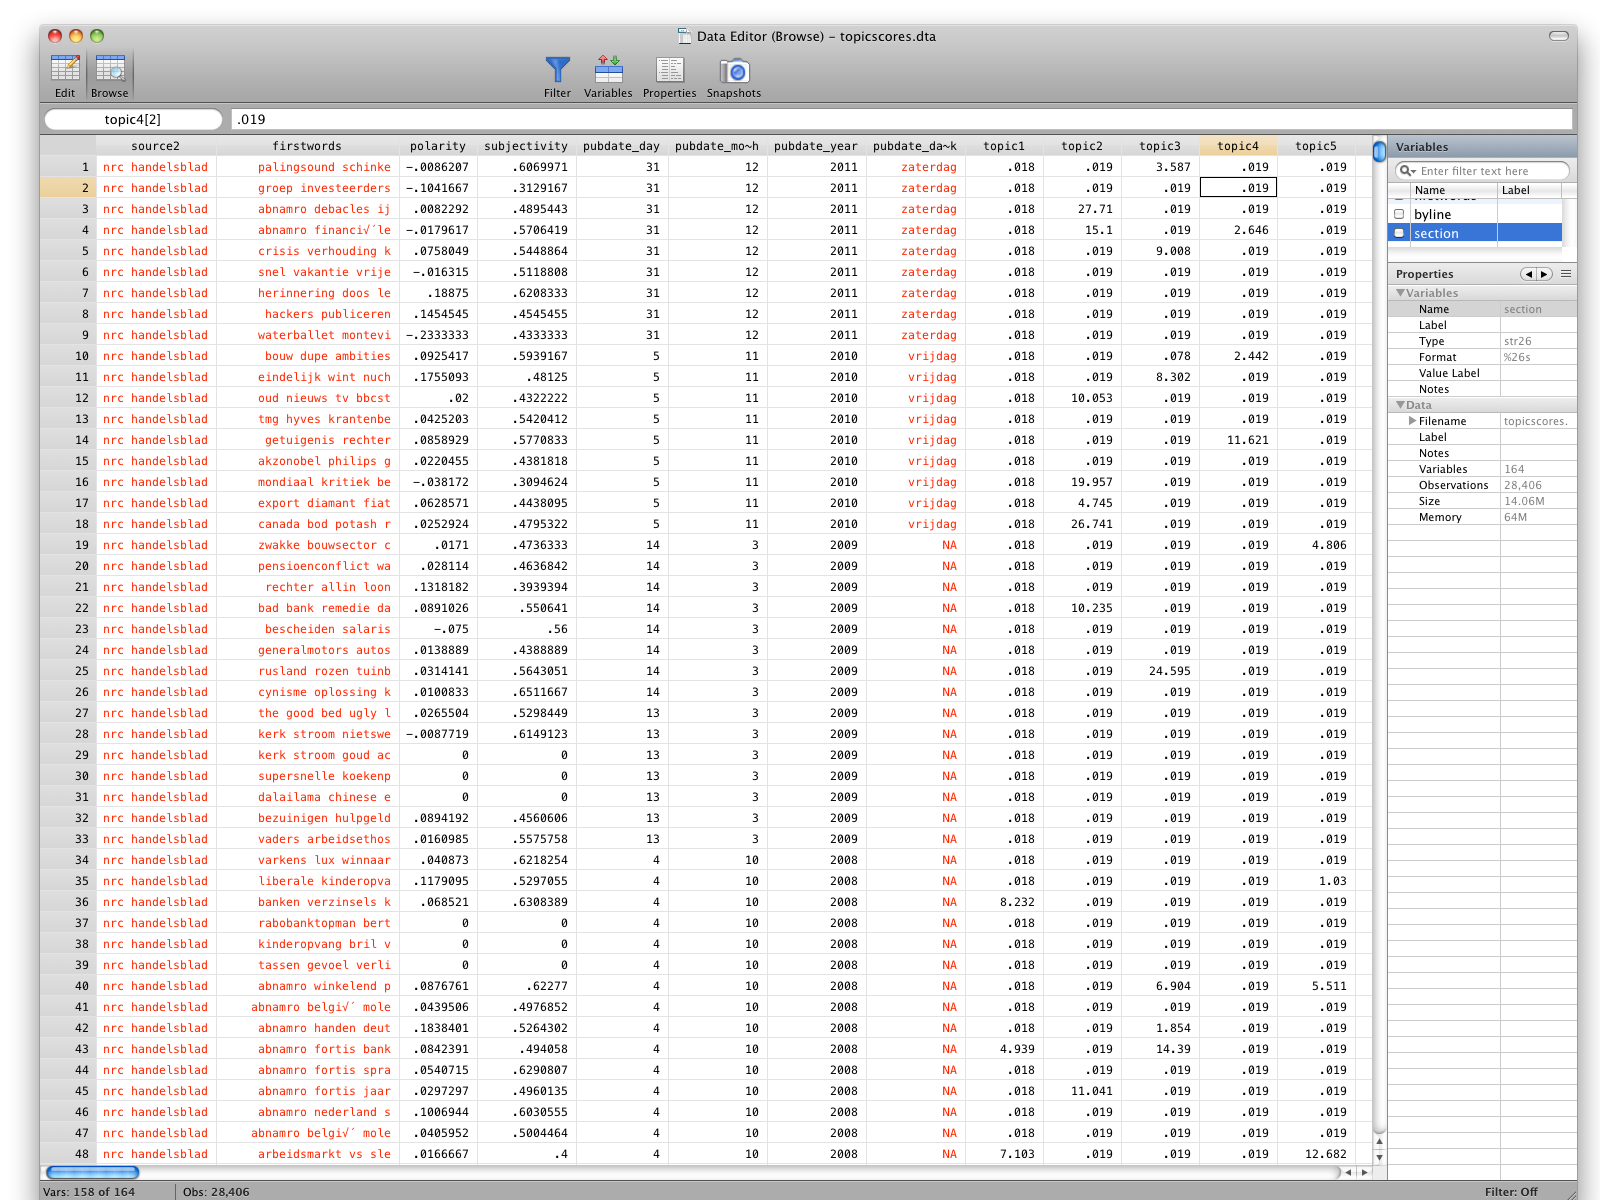
\includegraphics[width=\paperwidth,height=\paperheight,keepaspectratio]{../../pictures/topicscores}}
\end{frame}




\begin{frame}[fragile]{Visualization with pyldavis}
\begin{lstlisting}
import pyLDAvis
import pyLDAvis.gensim
# first estiate gensim model, then:
vis_data = pyLDAvis.gensim.prepare(mylda,mm,id2word)
pyLDAvis.display(vis_data)
\end{lstlisting}
\makebox[\linewidth]{
	\includegraphics[width=\paperwidth,height=.5\paperheight,keepaspectratio]{../../pictures/pyldavis}}
\end{frame}







\section[Supervised Machine Learning]{Supervised Machine Learning}

\begin{frame}[plain]
	predefined categories, but no predefined rules:\\ \textbf{supervised machine learning}\\
	\vspace{1cm}\hspace{1cm} \onslide<2> \footnotesize{(something you aready did in your Bachelor -- no kidding.)}
\end{frame}








\begin{frame}{Recap: supervised vs. unsupervised}
	\begin{columns}[t]
		
			\column{.5\textwidth}
			
			\begin{block}{Unsupervised}<1->
				\begin{itemize}
					\item No manually coded data
					\item We want to identify patterns or to make groups of most similar cases
					%\item Per case, we want to know to which group it belongs
				\end{itemize}
			\end{block}
			{\footnotesize{
					\onslide<2->{Example: We have a dataset of Facebook-massages on an organizations' page. We use clustering to group them and later interpret these clusters (e.g., as complaints, questions, praise, \ldots)}
				}}
				
\column{.5\textwidth}
\begin{block}{Supervised}<3->
	\begin{itemize}
		\item We code a small dataset by hand and use it to ``train'' a machine
		\item The machine codes the rest 
	\end{itemize}
\end{block}

{\footnotesize{
		\onslide<4->{Example: %We use a hand-coded CSV table with two columns (tweet and gender of the sender) as training dataset and then predict for a different dataset per tweet if it was sent by a man or a woman.
			We have 2,000 of these messages grouped into such categories by human coders. We then use this data to group all remaining messages as well.
			}
	}}

	\end{columns}
\end{frame}









\subsection{You have done it before!}
\begin{frame}{You have done it before!}
\begin{block}{Regression}<2->
	\begin{enumerate}
		\item<3-> Based on your data, you estimate some regression equation 	$y_i = \alpha + \beta_1 x_{i1} + \cdots + \beta_p x_{ip} + \varepsilon_i$
		\item<4-> Even if you have some \emph{new unseen data}, you can estimate your expected outcome $\hat{y}$!
		\item<5-> Example: You estimated a regression equation where $y$ is newspaper reading in days/week: $y = -.8 + .4 \times man + .08 \times age$
		\item<6-> You could now calculate $\hat{y}$ for a man of 20 years and a woman of 40 years -- \emph{even if no such person exists in your dataset}: \\
		$\hat{y}_{man20} = -.8 + .4 \times 1 + .08 \times 20 = 1.2$ \\
		$\hat{y}_{woman40} = -.8 + .4 \times 0 + .08 \times 40 = 2.4$
	\end{enumerate}
\end{block}	

\end{frame}


\begin{frame}{}
	\huge{This is\\ Supervised Machine Learning!}
\end{frame}

\begin{frame}{\ldots but\ldots}
	\begin{itemize}
		\item<1-> We will only use \emph{half} {\tiny{(or another fraction)}} of our data to estimate the model, so that we can use the other half to check if our predictions match the manual coding (``labeled data'',``annotated data'' in SML-lingo)
		\begin{itemize}
			\item<2->e.g., 2000 labeled cases, 1000 for training, 1000 for testing --- if successful, run on 100,000 unlabeled cases
		\end{itemize}
		\item<3-> We use many more independent variables (``features'')
		\item<4-> Typically, IVs are word frequencies (often weighted, e.g. tf$\times$idf) ($\Rightarrow$BOW-representation)
	\end{itemize}
\end{frame}


\subsection{Applications}

\begin{frame}{Applications}
\begin{block}<2->{In other fields}
\emph{A lot} of different applications
\begin{itemize}
\item from recognizing hand-written characters to recommendation systems
\end{itemize}
\end{block}

\begin{block}<3>{In our field}
It starts to get popular to measure latent variables
\begin{itemize}
\item frames
\item topics
\end{itemize}
\end{block}
\end{frame}



\begin{frame}{SML to code frames and topics}
\begin{block}{Some work by Burscher and colleagues}
\begin{itemize}
\item Humans can code generic frames (human-interest, economic, \ldots)
\item Humans can code topics from a pre-defined list 
\item<2->\textbf{But it is very hard to formulate an explicit rule} \\(as in: code as 'Human Interest' if regular expression R is matched)
\end{itemize}
\onslide<3>$\Rightarrow$ This is where you need supervised machine learning!
\end{block}
\tiny{Burscher, B., Odijk, D., Vliegenthart, R., De Rijke, M., \& De Vreese, C. H. (2014). Teaching the computer to code frames in news: Comparing two supervised machine learning approaches to frame analysis. \emph{Communication Methods and Measures, 8}(3), 190–206. doi:10.1080/19312458.2014.937527
\\
Burscher, B., Vliegenthart, R., \& De Vreese, C. H. (2015). Using supervised machine learning to code policy issues: Can classifiers generalize across contexts? \emph{Annals of the American Academy of Political and Social Science, 659}(1), 122–131.
}

\end{frame}





{\setbeamercolor{background canvas}{bg=black}
\begin{frame}[plain]
\makebox[\linewidth]{
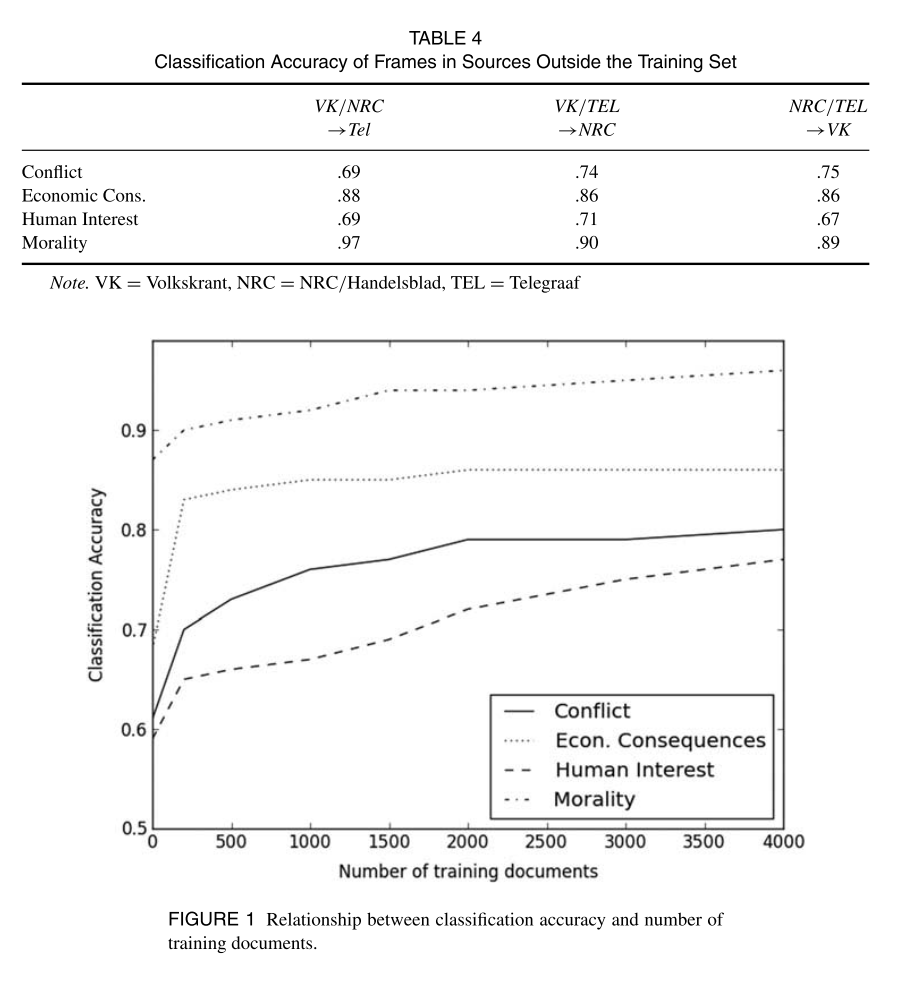
\includegraphics[width=\paperwidth,height=\paperheight,keepaspectratio]{../../pictures/burscher2014}}
\end{frame}

\begin{frame}[plain]
\makebox[\linewidth]{
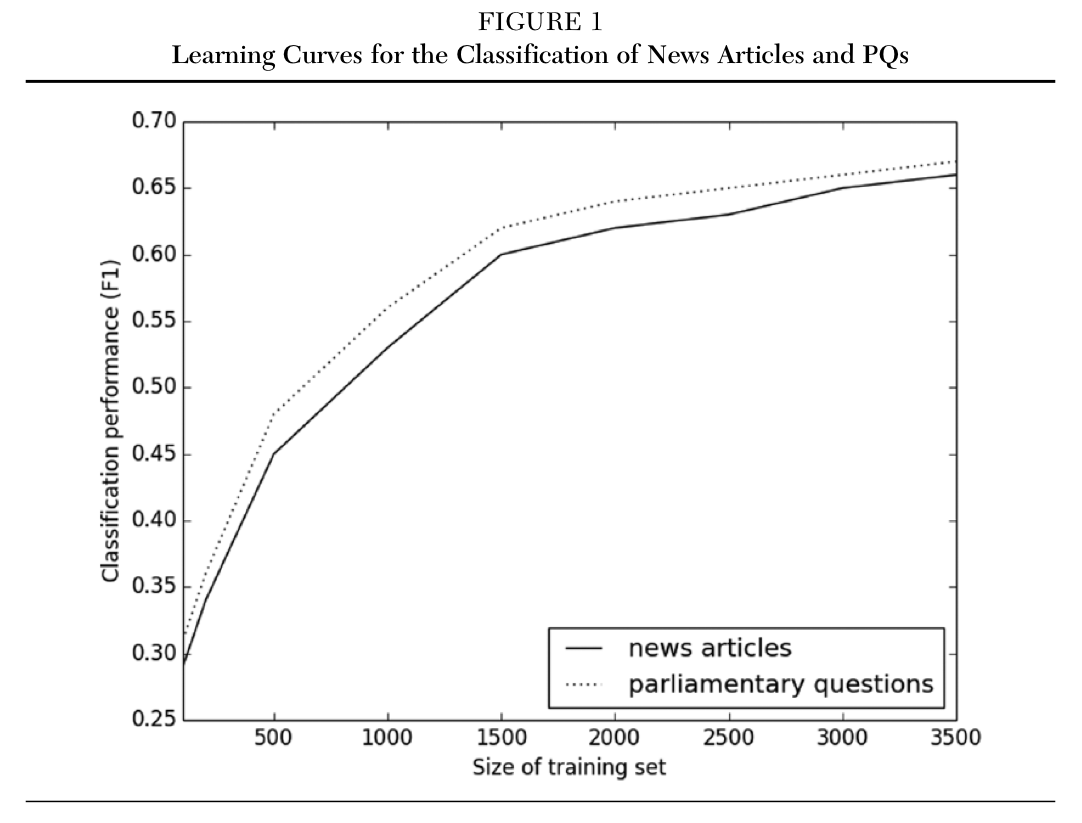
\includegraphics[width=\paperwidth,height=\paperheight,keepaspectratio]{../../pictures/burscher2015-a}}
\end{frame}

\begin{frame}[plain]
\makebox[\linewidth]{
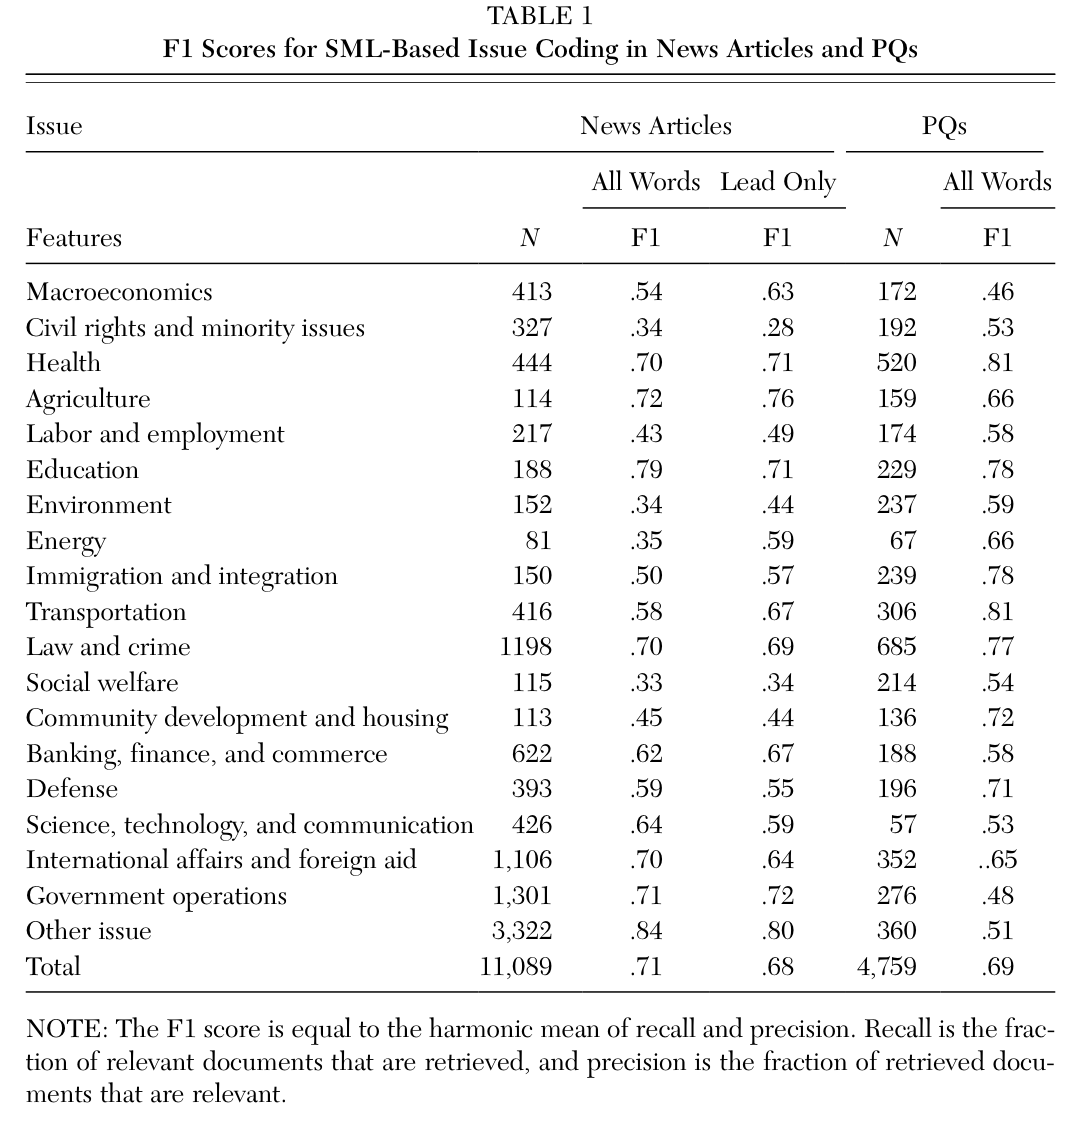
\includegraphics[width=\paperwidth,height=\paperheight,keepaspectratio]{../../pictures/burscher2015-b}}
\end{frame}
}

\begin{frame}[plain]
\begin{columns}[]
\column{.5\textwidth}

{\tiny{http://commons.wikimedia.org/wiki/File:Precisionrecall.svg}}
\makebox[\linewidth]{
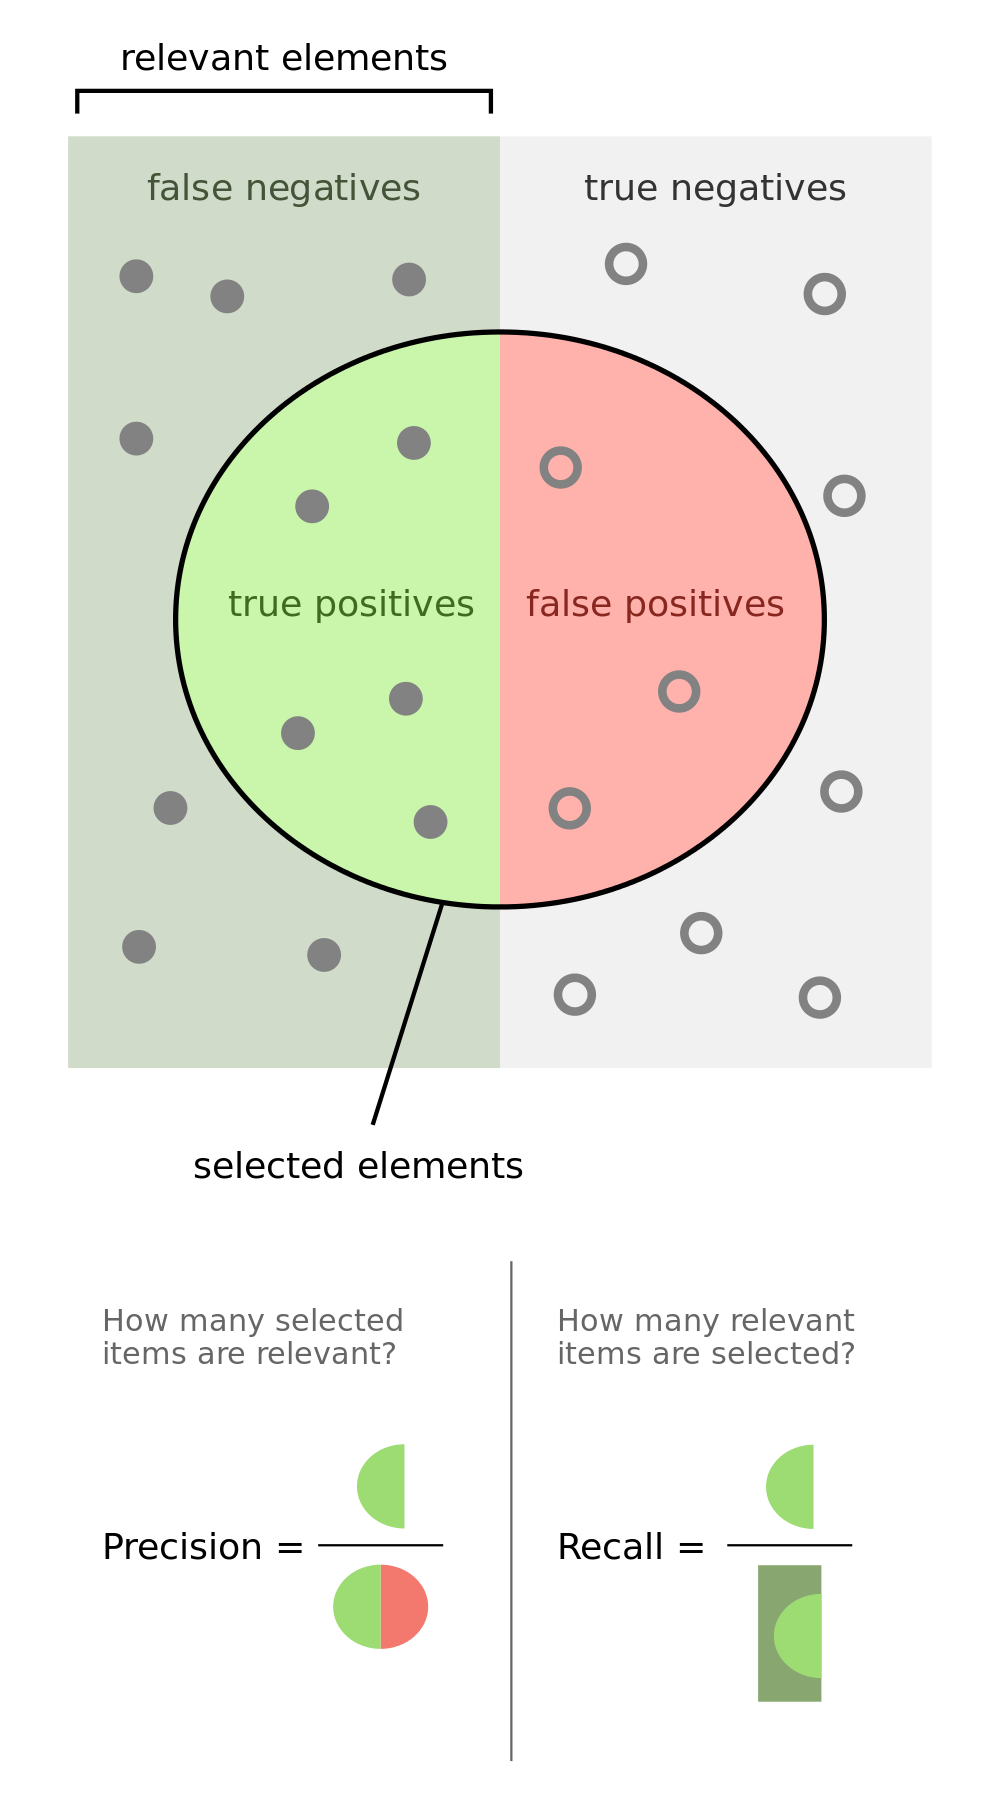
\includegraphics[width=\paperwidth,height=\paperheight,keepaspectratio]{../../pictures/precisionrecall.png}}

\column{.5\textwidth}
\begin{block}{Some measures of accuracy}
\begin{itemize}
\item Recall
\item Precision
\item $\text{F1}=2\cdot \frac{\text{precision}\cdot \text{recall}}{\text{precision}+\text{recall}}$
\item AUC (Area under curve) $[0,1]$, $0.5=$ random guessing
\end{itemize}
\end{block}


\end{columns}

\end{frame}





\begin{frame}{What does this mean for our research?}
\begin{block}<2>{It we have 2,000 documents with manually coded frames and topics\ldots}
\begin{itemize}
\item we can use them to train a SML classifier
\item which can code an unlimited number of new documents
\item with an acceptable accuracy
\end{itemize}
\end{block}
\onslide<2>{
\tiny{Some easier tasks even need only 500 training documents, see Hopkins, D. J., \& King, G. (2010). A method of automated nonparametric content analysis for social science. \emph{American Journal of Political Science, 54}(1), 229–247.}} 
\end{frame}



\subsection{An implementation}

\begin{frame}[fragile]{An implementation}
Let's say we have a list of tuples with movie reviews and their rating:
\begin{lstlisting}
reviews=[("This is a great movie",1),("Bad movie",-1), ... ...]
\end{lstlisting}
And a second list with an identical structure:
\begin{lstlisting}
test=[("Not that good",-1),("Nice film",1), ... ...]
\end{lstlisting}
Both are drawn from the same population, it is pure chance whether a specific review is on the one list or the other.\\
\tiny{Based on an example from \url{http://blog.dataquest.io/blog/naive-bayes-movies/}}
\end{frame}


\begin{frame}[fragile]{Training a A Naïve Bayes Classifier}
\begin{lstlisting}
from sklearn.naive_bayes import MultinomialNB
from sklearn.feature_extraction.text import CountVectorizer
from sklearn import metrics
 
# This is just an efficient way of computing word counts
vectorizer = CountVectorizer(stop_words='english')
train_features = vectorizer.fit_transform([r[0] for r in reviews])
test_features = vectorizer.transform([r[0] for r in test])
 
# Fit a naive bayes model to the training data.
nb = MultinomialNB()
nb.fit(train_features, [r[1] for r in reviews])
 
# Now we can use the model to predict classifications for our test features.
predictions = nb.predict(test_features)
actual=[r[1] for r in test]
 
# Compute the error.
fpr, tpr, thresholds = metrics.roc_curve(actual, predictions, pos_label=1)
print("Multinomal naive bayes AUC: {0}".format(metrics.auc(fpr, tpr)))

\end{lstlisting}
\end{frame}
%
%\begin{frame}{TODO}
%TODO\\
%andere vectorizer (TFIDF)\\
%verschillen classifiers\\
%andere output (metrics summary)
%\\
%waarom is dit hier een MULTINOMIAL NB
%\\
%scikit-learn installeren\\ 
%opdracht bedenken: classifiers vergelijken
%\end{frame}


\begin{frame}{And it works!}
Using 50,000 IMDB movies that are classified as either negative or positive,
\begin{itemize}
\item I created a list with 25,000 training tuples and another one with 25,000 test tuples and
\item trained a classifier
\item that achieved an AUC of .82.
\end{itemize}
~\\
\tiny{Dataset obtained from \url{http://ai.stanford.edu/~amaas/data/sentiment}, Maas, A.L., Daly, R.E., Pham, P.T., Huang, D., Ng, A.Y., \& Potts, C. (2011). Learning word vectors for sentiment analysis. \emph{49th Annual Meeting of the Association for Computational Linguistics (ACL 2011)}
}

\end{frame}

\begin{frame}[fragile]{Playing around with new data}
\begin{lstlisting}
newdata=vectorizer.transform(["What a crappy movie! It sucks!", "This is awsome. I liked this movie a lot, fantastic actors","I would not recomment it to anyone.", "Enjoyed it a lot"])
predictions = nb.predict(newdata)
print(predictions)
\end{lstlisting}
This returns, as you would expect and hope:
\begin{lstlisting} 
[-1  1 -1  1]
\end{lstlisting}


\end{frame}




\begin{frame}{But we can do even better}
	We can use different vectorizers and different classifiers.
\end{frame}

\begin{frame}{Different vectorizers}
	\begin{itemize}
		\item CountVectorizer (=simple word counts)
		\item TfidfVectorizer (word counts (``term frequency'') weighted by number of documents in which the word occurs at all (``inverse document frequency''))
		\item additional options: stopwords, thresholds for minimum frequencies etc.
	\end{itemize}
\end{frame}

\begin{frame}{Different classifiers}
	\begin{itemize}
		\item Naïve Bayes
		\item Logistic Regression
		\item Support Vector Machine (SVM)
		\item \ldots
	\end{itemize}
Typical approach: Find out which setup performs best (see example source code in the book).
\end{frame}





\section{Next meetings}
\begin{frame}{Next (last\ldots) meetings}
\begin{block}{Friday}
Playing around with machine learning! Choose what you find interesting (SML or LDA).
\end{block}

\begin{block}{Wednesday: Looking back and forward }
Putting in perspective what we have done. Putting all pieces together. Going forward: other techniques to use in your future projects.
\end{block}


\begin{block}{Friday}
	Final chance for questions regarding final project
\end{block}


\end{frame}




\end{document}

